\documentclass{article}
\usepackage{graphicx} 
\usepackage{tikz}
\usepackage{amsmath}
\usetikzlibrary{arrows.meta}
\usepackage{listings}
\usepackage{xcolor}
\usepackage{caption}

\lstdefinestyle{wsl}{
  backgroundcolor=\color{black},
  basicstyle=\color{white}\ttfamily,
  numbers=left,
  numbersep=5pt,
  frame=single,
  rulecolor=\color{gray},
  framexleftmargin=15pt,
  numberstyle=\tiny\color{gray},
  breakatwhitespace=false,
  breakindent=0pt,
  breakautoindent=false,
  breaklines=true
}


\title{Simulazione del moto di un punto materiale in un biliardo triangolare}
\author{Sabattini Manginella Cesare \\
Tonti Mattia}
\date{17 Maggio 2024}

\begin{document}

\maketitle

\section*{Source Code}
Il source code è reperibile presso:
\\git@github.com:CesareSabattini/Triangular\_Billiard.git

\section{Abstract}
Il programma è volto alla simulazione di collisioni multiple e sequenziali di un punto materiale contro le pareti
di un biliardo triangolare, con lo specifico obiettivo di studiare la distribuzione delle ordinate e degli angoli di uscita.
L'applicazione è provvista di modulo di simulazione e modulo di analisi, il tutto implementato secondo lo standard ISO C++20, con l'ausilio del framework SFML 2.6 per la realizzazione della GUI.

\section{Introduzione}


\begin{figure}[ht]
    \centering
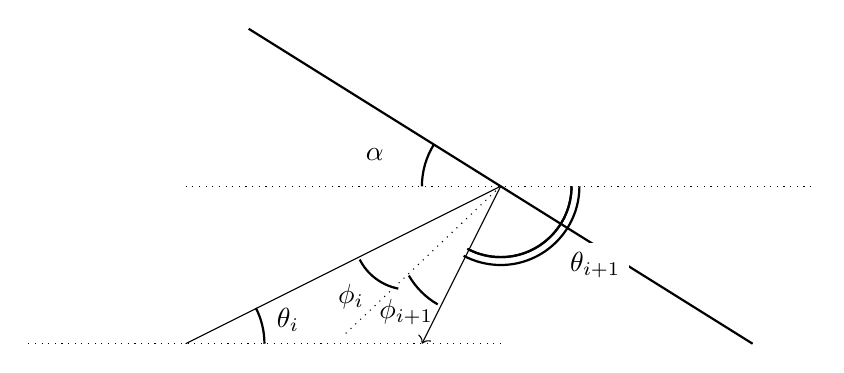
\begin{tikzpicture}

\draw[thick] (-0.2,2) -- (6.2,-2);
\draw[dotted] (-1,0) -- (7,0);
\draw[dotted] (-3,-2) -- (3,-2);
\draw (-1,-2) -- (3,0);
\draw[->] (3,0) -- (2,-2);
\draw[dotted] (3,0) -- (1,-1.9);

\draw[thick] (2,0) arc[start angle=180,end angle=148,radius=1];
\draw[thick] (0,-2) arc[start angle=0,end angle=27,radius=1];
\draw[thick] (4,0) arc[start angle=0,end angle=-118,radius=1];
\draw[thick] (3.9,0) arc[start angle=0,end angle=-118,radius=0.9];
\draw[thick] (3.9,0) arc[start angle=0,end angle=-118,radius=0.9];
\draw[thick] (2.2,-1.5) arc[start angle=-120,end angle=-150,radius=1];
\draw[thick] (1.7,-1.3) arc[start angle=-101,end angle=-153,radius=0.7];

\node at (1.4,0.4) {$\alpha$};
\node at (0.3,-1.7) {$\theta_i$};
\fill[white] (4.1,-1.1) rectangle (4.5,-0.9);
\node[fill=white] at (4.2, -1) {$\theta_{i+1}$};
\node at (1.1,-1.4) {$\phi_i$};
\node at (1.8,-1.6) {$\phi_{i+1}$};

\end{tikzpicture}
    \caption{
    \centering
Modello di urto elastico punto-parete, riportante notazioni secondo le convenzioni scelte nell'analisi del problema.
    }
    \label{fig:wavefront}

\end{figure}
Dato un urto elastico, vale:

\begin{equation}
    \phi_i=\phi_{i+1}
\end{equation}

Definito \(\alpha\) l'angolo di inclinazione delle pareti,

\begin{equation}
\alpha=\arctan{\left(\frac{R_1-R_2}{L}\right)}\\
\end{equation}

a seguito dell'urto i-esimo, per i$>$0 \footnote{Viene considerato come urto 0, il lanco del punto materiale.}, vale

\begin{equation}
\centering
\theta_{i+1}=-(|\theta_{i}|+2\alpha) 
\end{equation}

Per i=0 vale\\
\begin{equation}
\left\{
\begin{aligned}
    & |\theta_1|=2\alpha-|\theta_0| \hspace{2.5 mm} se\hspace{2.5 mm}|r_2|<|y|<|r_1|,\hspace{2.5 mm} \theta_0<\alpha ,\hspace{2.5 mm}  y_0\theta_0<0  \\
    & \theta_1=-(|\theta_i|+2\alpha) \hspace{2.0mm} altrimenti
\end{aligned}
\right.
\end{equation}\\

Le coordinate della collisione i+1 sono date dal sistema lineare

\begin{equation}
\left\{
\begin{aligned}
   & y_{i+1}=y_i+\tan\theta_i \cdot (x_{i+1}-x_i) \\
   & |y_{i+1}|= R_1 - \tan\alpha \cdot x_{i+1}
\\
\end{aligned}
\right.
\end{equation}


Date n simulazioni indipendenti, si analizzano le distribuzioni di $y_f$ e $\theta_f$ .

Le coordinate $y_i$ e $\theta_i$ sono generate secondo distribuzioni gaussiane:

\begin{equation}
    f(x) = \frac{1}{\sigma\sqrt{2\pi}} e^{-\frac{(x-\mu)^2}{2\sigma^2}}
\end{equation}

con media \(\mu\) e deviazione standard \(\sigma\).
Delle distribuzioni esito si computano:
\begin{itemize}
    \item media:

\begin{equation}
    \mu = \frac{1}{N} \sum_{i=1}^N x_i
\end{equation}

\item deviazione standard della media:
\begin{equation}
    \sigma_m = \frac{\sigma}{\sqrt{N}} = \frac{\sqrt{\frac{1}{N-1} \sum_{i=1}^N (x_i - \mu)^2}}{\sqrt{N}}
\end{equation}



\item coefficiente di simmetria:
\footnote{Si utilizza il coefficiente di Fisher-Pearson ottimizzato.}

\begin{equation}
    \gamma_1 = \frac{\sqrt{N\cdot (N-1)}}{N(N-2)} \sum_{i=1}^N \left(\frac{x_i - \bar{x}}{s}\right)^3
\end{equation}

\item coefficiente di appiattimento:

\begin{equation}
   \gamma_2 =  \frac{1}{N}\sum_{i=1}^N \left(\frac{x_i - \bar{x}}{s}\right)^4 - 3
\end{equation}
\end{itemize}


\section{Struttura del codice}
Si discute di seguito la struttura del codice secondo l'organizzazione dei namespaces.

\subsection{Simulation}
Si implementano le classi necessarie per la logica della simulazione.
I templates sono vincolati dal concept minimale DoubleOrFloat, che verifica al compiletime un constrain di tipo.
\begin{itemize}
    \item $Ball$ contiene le informazioni relative a posizione e angolo di inclinazione della propria traiettoria.
    \item $Pool$ conserva i parametri strutturali del biliardo: r1 (metà della base maggiore), r2 (metà della base minore),
    l (lunghezza).
    \item $Collision$ possiede le informazioni sulla posizione e sull'angolo di riflessione di una collisione.
    \item $System$ funge da interfaccia di gestione del sistema: contiene una $Ball$, un $Pool$ e un vettore di $Collision$.
    Il metodo updateParams() inizializza $Pool$ e $Ball$, simulate() esegue una simulazione, riempiendo il vettore di collisioni.
    Il metodo $computeOutputY()$ restituisce $y_f$, mentre $\theta_f$ si ricava dall'ultima collisione.

\end{itemize}

\subsection{Analysis}

Si implementano le strutture necessarie per l'analisi delle distibuzioni di $y_f$ e $\theta_f$.
\begin{itemize}
    \item $Parameters$ contiene i parametri di inizializzazione di ogni simulazione: media e sigma delle gaussiane di $y_i$ e $\theta_i$, e numero di simulazioni.
    \item $Results$ raggruppa i risultati dell'analisi.
    \item $Analyzer$ contiene un puntatore condiviso ad un'istanza di $System$. \\
    Mediante std::random\_device e std::mt19937 \footnote{generatore di numeri casuali provvisto dalla Standard Library, basato sull'algoritmo Marsenne Twister}, $generate()$ inizializza il vettore $inputs$, secondo quanto contenuto in $Params$.\\
    $simulate()$ effettua un numero di simulazioni pari a $Params::numSimulations$, ed inizializza il vettore $outputs$.\\
    $analyze()$ inizializza $Results$.
    
\end{itemize}

\subsection{Graphics}
Si implementa la GUI servendosi del framework SFML 2.6.\\
La grafica è logicamente suddivisa in $scenes$ (finestre grafiche) e $components$ (componenti condivisi dalle scenes).\\
La classe MainWindow funge da interfaccia di rendering: tramite switch block condizionale secondo un valore della enum class $Scene$, viene mostrata una finestra specifica.\\
Inoltre essa contiene un puntatore condiviso a $System$, così da garantirne la proprietà condivisa e leak-free con ogni $scene$.

\subsubsection{Scenes}
Ogni $scene$ implementa i canonici metodi di rendering di SFML, volti al drawing e alla gestione degli eventi ($initializeComponents()$, $draw()$ e $processEvents()$)\footnote{$initializeComponents()$ effettua semplicemente la configurazione delle componenti grafiche(dimensioni, posizionamento, colore, ...), perciò se ne omette qui una descrizione approfondita.}

\begin{itemize}
    \item $Menu$ è la UI mostrata all'avvio dell'applicazione, e conduce alle interfacce di configurazione della simulazione singola e a quella di analisi.
    \item $ConfigSimulation$ permette di configurare una singola simulazione e di avviarla: cliccando $startButton$, si inizializza il sistema e si avvia la simulazione.
    \item $SimulationWindow$ restituisce una rappresentazione grafica minimale della traiettoria del punto materiale, utilizzando le coordinate delle collisioni, contenute nel vettore $System::collisions$.
    \item $AnalysisWindow$ consente l'inserimento dei dati necessari per l'analisi statistica di simulazioni multiple. \\ Cliccando $analyzeButton$ si inizializza un $Analyzer$ al contenuto dei $textInputs$ e si avvia il processo di analisi. Al termine, si riempiono le labels con i risultati in output.
\end{itemize}

\section{Error Handling}
Si è optato per le eccezioni come meccanismo principale di runtime error handling.
Il ciclo di rendering di MainWindow è inserito in un blocco try-catch, che cattura tutte le eccezioni provenienti dalle componenti grafiche. Il catch le cattura e mostra a schermo una minimale finestra di pop up, contenente il messaggio di errore.\\
Le eccezioni sono lanciate in tutti i costruttori delle classi di simulazione, qualora non siano verificati i requisiti logici di inizializzazione al runtime.
Questo meccanismo è stato anche usato per gestire la logica di $System::simulate()$.


\section{Gestione delle Risorse}
Le risorse sono organizzate al fine di minimizzare operazioni dispendiose non necessarie.
Sia nella grafica, che nel testing, per esempio, si è fatto ampio uso di std::shared\_ptr per la gestione di oggetti di tipo System, al fine di mantenere la stessa istanza condivisa.
Analogamente per il font, evitando uploads multipli.\\
Le operazioni di copia sono minime, e limitate a tipi primitivi del linguaggio.
E' stata inoltre prestata molta attenzione alla const correctness.


\section{Testing}
Si organizzano due macro di testing con Doctest, per simulazione e analisi.
Si implementa in aggiunta la classe $MockSystem$, che effettua l'override del metodo $System::simulate()$, rimuovendone i loggers, per non interferire con l'interfaccia di testing.

\section{Compilazione}
Il documento CMake compila $core\_lib$, libreria dinamica linkata agli eseguibili $Triangular\_Pool$ e $tests$.\\
Le flags di compilazione includono le opzioni richieste per la rilevazione di warnings.\\
È definita inoltre l'opzione $ENABLE\_SANITIZERS$, che permette di abilitare il supporto di Address Sanitizer al run-time.\\
Se attiva, vengono aggiunte le appropriate flags per abilitare i sanitizzatori.

\subsection{Istruzioni di compilazione}
Per la compilazione su LinuxOS e WSL si raccomanda di seguire i seguenti passaggi:


\begin{itemize}
    \item Installare le dipendenze necessarie:
    \begin{lstlisting}[style=wsl]
sudo apt update
sudo apt install build-essential cmake libsfml-dev
\end{lstlisting}

\item Per compilare l'eseguibile $Triangular\_Pool$ in modalità Debug con Address Sanitizer:
    \begin{lstlisting}[style=wsl]
cmake -B build/debug -DCMAKE_BUILD_TYPE=Debug -DENABLE_SANITIZERS=ON
cmake --build build/debug --target Triangular_Pool
\end{lstlisting}

\item Per compilare l'eseguibile $tests$ in modalità Debug con Address Sanitizer:
    \begin{lstlisting}[style=wsl]
cmake -B build/debug -DCMAKE_BUILD_TYPE=Debug -DENABLE_SANITIZERS=ON
cmake --build build/debug --target tests
\end{lstlisting}

\item Per compilare l'eseguibile $Triangular_Pool$ in modalità Release:
    \begin{lstlisting}[style=wsl]
cmake -B build/release -DCMAKE_BUILD_TYPE=Release -DENABLE_SANITIZERS=OFF
cmake --build build/release --target Triangular_Pool
\end{lstlisting}


\item Per compilare l'eseguibile $tests$ in modalità Release:
    \begin{lstlisting}[style=wsl]
cmake -B build/release -DCMAKE_BUILD_TYPE=Release -DENABLE_SANITIZERS=OFF
cmake --build build/release --target tests
\end{lstlisting}




\item Per avviare l'eseguibile dalla directory build:
    \begin{lstlisting}[style=wsl]
./Triangular_Pool
\end{lstlisting}

\item Per eseguire il testing:
    \begin{lstlisting}[style=wsl]
./tests
\end{lstlisting}

\end{itemize}


\section{Bibliografia e sitografia}

\begin{itemize}
    \item Bjarne Stroustrup, "C++. Linguaggio, libreria standard, principi di programmazione", 2019, Pearson.
    \item SFML 2.6, https://www.sfml-dev.org/tutorials/2.6/
    \item Microsoft Learn, https://learn.microsoft.com/it-it/cpp/?view=msvc-170, per i seguenti temi:
    \begin{itemize}
        \item Generazione di numeri casuali (https://learn.microsoft.com/it-it/cpp/standard-library/random?view=msvc-170).
        \item Implementazione di template classes tra .hpp e .cpp:
        https://learn.microsoft.com/en-us/cpp/cpp/source-code-organization-cpp-templates?view=msvc-170
    \end{itemize}
      \item Per le definizioni utilizzate di coefficienti di simmetria ed appiattimento, NIST, https://www.nist.gov/

      \item DOCtest 2.4.11, https://github.com/doctest/doctest
      \item cppreference, https://en.cppreference.com/w/, prevalentemente per la Standard Library e concepts.
      \item Angular convectional commit, https://www.conventionalcommits.org/en/v1.0.0-beta.4/   
\end{itemize}

\end{document}
